\documentclass[border=10pt]{standalone}
\usepackage{tikz}
\usetikzlibrary{calc,positioning,shadows.blur,decorations.pathreplacing}
\usepackage{etoolbox}
\usepackage{graphicx}
\usepackage{amsmath}
\graphicspath{{figures/}}


\begin{document}
	\begin{tikzpicture}
	
	%begin by adding a node for each figure
	\node[inner sep=0pt] (imgs) at (0,0)
		{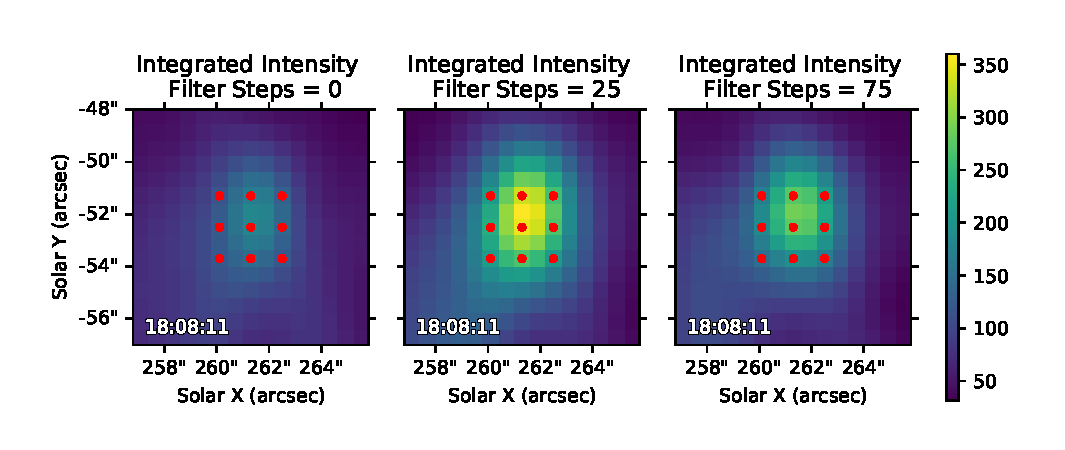
\includegraphics[]{perfectx_invert_comp_a}};
	\node[inner sep=0pt] (lps) at (0,-11)
		{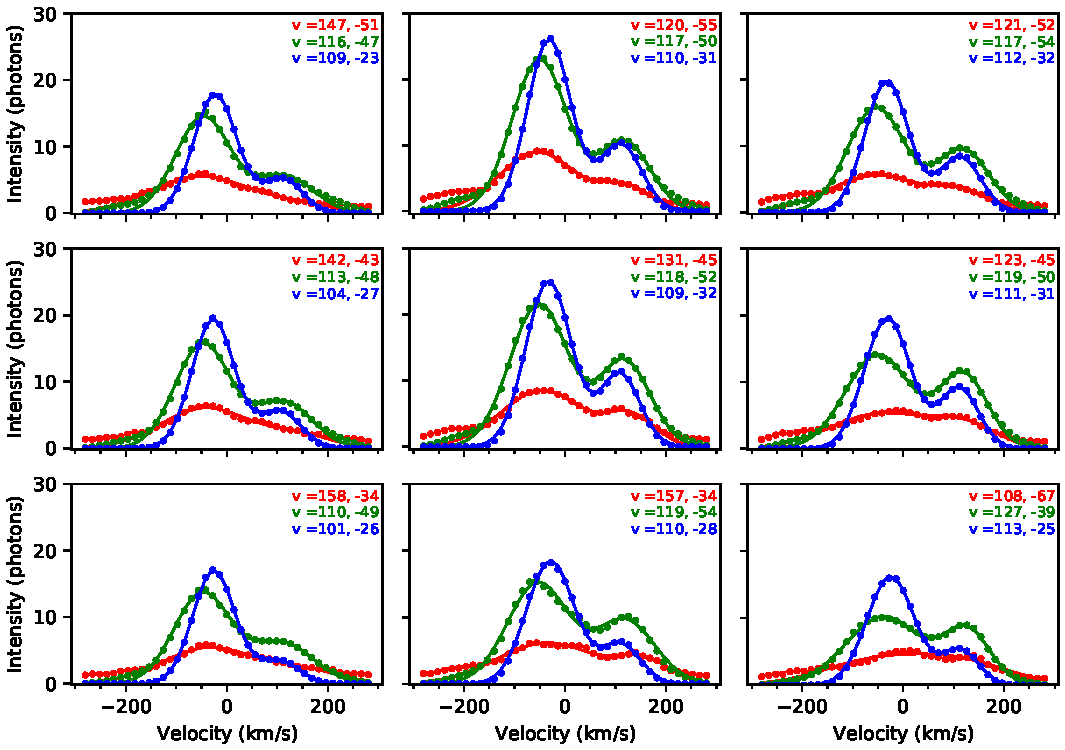
\includegraphics[]{perfectx_invert_comp_b}};
	

	\end{tikzpicture}
\end{document}